\RequirePackage[l2tabu,orthodox]{nag}
\documentclass{article}
%\pdfoutput=1
\pdfminorversion=4
\let\columnlines\empty
\usepackage{times}
\usepackage{amsmath}
\usepackage{amssymb}
\usepackage{latexsym}
\usepackage{graphicx}
\usepackage{subfigure} 
\usepackage{url}
\usepackage[stretch=10]{microtype}
\usepackage{todonotes}
\usepackage{natbib}
\usepackage[hyperfootnotes=false,hidelinks=true]{hyperref}
\usepackage{multirow}

\title{Test Case for Converters from \LaTeX to Word Processor Format}
\author{}

\begin{document}
\maketitle

%%%%%%%%%%%%%%%%%%%%%%%%%%%%%%%%%%%%%%%%%%%%%%%%%%%%%%%%%%%%%%%%%%%%%%%
\section{Introduction}
Mathematical formulae are the nemesis of converters. This is a simple inline equation: $x=2$. This one contains a fraction: $y=\frac{1}{2}$. The following one has a subscript: $z_{1}=t$. Here goes a summation: $\sum_{i=0}^{\infty}a_{i}^{2}$.

The following is a simple equation:
\begin{equation}
  \sum_{i=0}^{\infty}a_{i}^{2}.
\end{equation}

This equation includes the identity operator from amssymb:
\begin{equation}
  \sum_{i}\Pi_{i}=\mathbb{I}.
\end{equation}

Whereas the following one includes a pmatrix from amsmath:
\begin{equation}
  e_{1}=\begin{pmatrix} 1 \\ 0 \\ 0 \\ 0 \\ 0 \\0 \end{pmatrix}.
\end{equation}

The same column vector is expressed as an array in math mode:
\begin{equation}
  e_{1}=\left(\begin{array}{c} 1 \\ 0 \\ 0 \\ 0 \\ 0 \\0 \end{array}\right).
\end{equation}

This is a cross reference to the next section: Section~\ref{figures}

This is a citation without parenthesis: \cite{dummy2013least}. The citation after this sentence should have parenthesis if natbib works correctly~\citep{dummy2013least}

%%%%%%%%%%%%%%%%%%%%%%%%%%%%%%%%%%%%%%%%%%%%%%%%%%%%%%%%%%%%%%%%%%%%%%%
\section{Figures and tables}\label{figures}
\begin{figure}[ht!]
  \begin{center}
      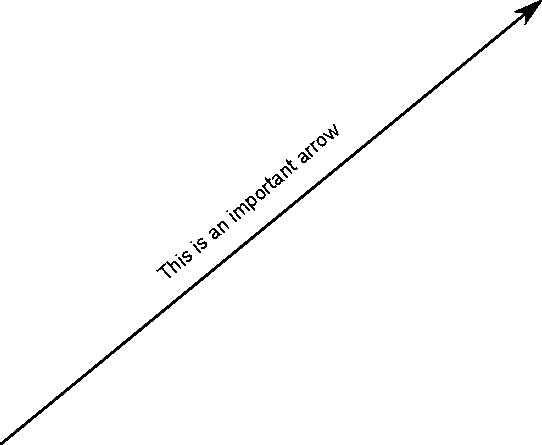
\includegraphics[width=0.3\textwidth]{figures/arrow.pdf}
    \caption{Arrow included in PDF format.}
    \label{arrowpdf}
  \end{center}
\end{figure}

\begin{figure}[ht!]
  \begin{center}
      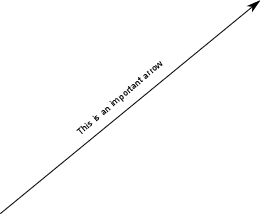
\includegraphics[width=0.3\textwidth]{figures/arrow.png}
    \caption{Arrow included in PNG format.}
    \label{arrowpng}
  \end{center}
\end{figure}

\begin{figure}[ht!]
\centering
\subfigure[PDF]{
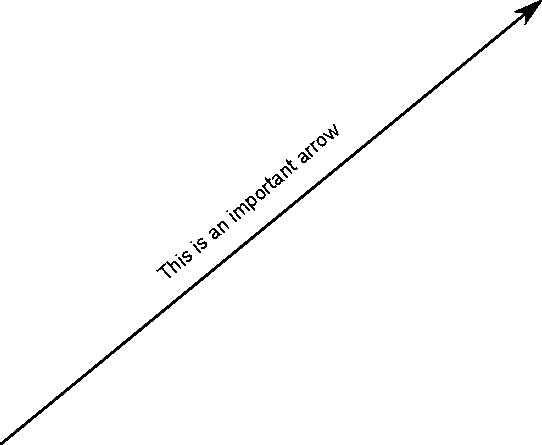
\includegraphics[width=0.3\textwidth]{figures/arrow.pdf}
}
\subfigure[PNG]{
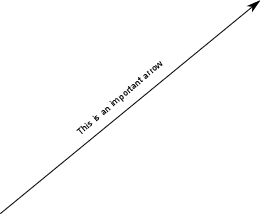
\includegraphics[width=0.3\textwidth]{figures/arrow.png}
}
\label{combined}
\caption{Images combined in subfigure environment.}
\end{figure}

Figure~\ref{arrowpdf} includes an arrow in PDF format. Figure~\ref{arrowpng} includes the same image bitmapped in PNG format. Figure~\ref{combined} combined the two images in a subfigure environment.

\begin{table}
\begin{center}
\begin{tabular}{c|c|c}
Column 1 & Column 2 & Column 3\\
\hline
1&2& $x^{2}$\\
\hline
\end{tabular}
\caption{Simple table.}
\label{simple}
\end{center}
\end{table}

\begin{table}
\begin{center}
\begin{tabular}{|c|c|c|}
\hline
\multirow{2}{*}{Multirow}&\multicolumn{2}{|c|}{Multicolumn}\\
\cline{2-3}
&I&II\\
\hline
1&2& $x^{2}$\\
\hline
\end{tabular}
\caption{Complicated table.}
\label{complicated}
\end{center}
\end{table}

Table~\ref{simple} is a simple table without requiring special packages. Table~\ref{complicated} is more complicated: it includes multiple rows and multiple columns.

\bibliographystyle{apalike}
\bibliography{bibliography}

\end{document}
